Throughout the course of these experiments, we have learned a number of lessons pertaining to the behavior of Spark for linear algebra computations in large scale HPC systems. 
In this section, we share some of these lessons and conjecture on likely causes.
\subsection{Spark Scheduling Bottlenecks}

\begin{table}[th]
\begin{center}
\resizebox{\columnwidth}{!}{
\begin{tabular}{| c | c | c | c | c | c | c |}
\hline
Algo & Size & Nodes & Partitions & Time (s) & Measured & Predicted \\
{} & {} & {} & {} & {} & Task Start & Delay \\
{} & {} & {} & {} & {} & Delay (s) & (2000/sec) \\
\hline
%\multirow{3}{*}{NMF} & \multirow{3}{*}{1.6 TB} & 
% 50 & 3200 & 710 & & \\
% {} & {} & 100 & 3200 & 457 & & \\
% {} & {} & 300 & 9600 & 215 & & \\ %\hline
\multirow{4}{*}{PCA} & \multirow{3}{*}{2.2 TB} & 100 & 3200 & 924 & 411 & 112 \\
 {} & {} & 300 & 9600 & 827 & 332 & 336 \\
 {} & {} & 500 & 16000 & 1160 & 542 & 560 \\ \cline{2-7} & & & & & & \\[-1ex]
 {} & {16 TB} & 1522 & 51200 & 3718 & 1779 & 1792 \\
 \hline
\end{tabular}
}
\end{center}
\caption{Spark scheduling delays}
\label{tab:scheduling}
\end{table}
%There are two main sources of sequential bottleneck in Spark: Task Start Delay and Scheduler Delay. Task Start delay for a particular task is the time from the start of the stage to when the scheduler creates and sends out the task to an executor. Because tasks are created one by one by the driver as it checks resources to see where to send them, higher concurrency leads to high task start delays. Scheduler delay consists of two items: the time it takes for the executor to receive the message to start as task and spawn a thread and the time it takes for the task to send a message back to the driver. Scheduler delay is known to be either caused by large tasks or large results, which slow down the sending process. In our case, however, we believe that a big part of the scheduler delay we observe increasing as we increase concurrency is due to the large number of tasks we are launching at once. This causes delay as many task completed messages are sent back to the driver at once and are queued as they are processed one by one. 
The Spark driver creates and sends tasks serially, which can cause bottlenecks at high concurrency.  This can be measured by looking at two metrics: Task Start Delay and Scheduler Delay. Task Start Delay measures the time until the  task is sent to an executor. Scheduler Delay measures the additional time until the driver receives confirmation that the task has been received and begun execution.  In figure~\ref{fig:hero-timeline}, we show a plot of a sample of tasks from one stage of the PCA hero run.  Note that the ordering of the colored bars within each task line does not correspond to the order they occurred---Spark uses a pipelined execution model, where different portions of a task are interleaved at a fine grain, and then reports back total times spent on each activity.  We can see that this scheduling bottleneck causes a uniform distribution of start times, with tasks starting as late as 20 seconds after the earliest task.  The scheduler delay appears inversely proportional to start delay, indicating that confirmation messages are queuing up and waiting to be processed at the driver while it finishes sending new tasks.

%Interestingly enough, the tasks finish at about the same time, as the scheduler delay seems to inversely proportional to the start delay. 

%Despite this strange behavior, it is clear that this delay negatively affects task performance. 

Ousterhout et al.~\cite{Ousterhout13Sparrow} showed that these factors limit the Spark scheduler to launching approximately 1500 tasks per second.  Their measurements were based on an older version of Spark from 2013.  There have not been significant changes to the scheduler, however, and our results on Cori are consistent with a similar rate of about 2000 tasks per second.  We show the impact of this bottleneck on PCA in Table~\ref{tab:scheduling}.  
We expect the largest impact on scaling here, due to the need to schedule 70 iterations.  Each iteration contains an initial stage that must schedule a task for every partition.  The \emph{Measured Task Start Delay} column shows the sum of the largest task start delays in each Spark stage.  The \emph{Predicted Delay} column shows the delay predicted by a scheduling rate of 2000 tasks per second over 70 iterations and the listed number of tasks/partitions.  We observe that at 300, 500, and 1522 nodes, the task start delay is very close to the predicted~value.\footnote{At 100 nodes, we see a delay that is much higher than predicted, indicating that an additional source of delay has contributed.  In particular, there was a single task with a delay of 90 seconds during that run, which alone accounts for almost a third of the difference from the predicted value.}

This bottleneck represents a limit on the scaling achievable by Spark for highly iterative algorithms.  In particular, as the amount of parallelism increases, the minimum number of partitions and tasks also increases.  This results in a linearly increasing overhead from the scheduler as we increase parallelism.  This delay is further multiplied by the number of stages.  We see the impact of this in the PCA results in Table~\ref{tab:scheduling}, where the final column represents this fixed overhead and is thus a lower bound on how fast we can execute at the given scale.  
\subsection{Other Significant Spark Overheads}
In figures \ref{fig:nmfspark} and \ref{fig:sparkpca}, we see a large block of time spent in Task Overheads. These consist of  shuffle read and write time, task deserialization time (Executor Deserialize Time), and result serialization time.  During our runs on Cori, most of these are insignificant with the exception of Executor Deserialize time, which can be seen in  figure~\ref{fig:whisker}.  High Executor Deserialize time is usually caused by large tasks that take a long time to unpack. Also, any garbage collection time occuring during the deserialize phase counts toward the deserialize time.
\subsection{Spark Variability/Stragglers}
The Time Waiting for Stage to End bucket describes the idle time in which a task has finished, but the next stage has not started, so new tasks have not yet been scheduled. The main cause of this idle time is ``straggler" tasks, tasks that take a longer than average time to finish and thus hold up the next stage from starting. In figure~\ref{fig:whisker}, we can see there is some variability in multiply Gramian component of tasks, but that is insignificant compared to the Spark overheads: Scheduler and Task Start Delay, as well as Task Deserialization time. These overheads vary anywhere from less than a second to more than 20 seconds. This variation in task behavior leads to some task slots left idle for up to 10 seconds.

The globally-synchronized execution model of Spark creates scaling issues in the presence of stragglers. When a small number of tasks take much longer to complete, many cores end up stuck idling at barriers. At larger scales, we see increases in both the probability of at least one straggler, as well as the number of underutilized cores waiting at barriers.


% During initial testing runs of the Spark PCA algorithm, variations in run time as large as 25\% were observed (in our staging runs we had a median run time of 645 seconds, a minium run time of 489 seconds, and a maximum run time of 716 seconds). These variations could not be attributed to any particular spark stage. Sometimes the delay would occur in the Multiply Gramian step, other times in the intial data collect stage. This variability is illustrated in the box and whiskers plot. Spark has a ``speculation" functionality which is aimed at reducing this variability somewhat. However, we found that turning the functionality on had no appreciable effect on improving the run time because the overhead to fetch an RDD from another worker was sufficiently high. This is because requests for RDDs from other workers must wait until the worker finishes its running tasks. This can often result in delays that are as long as the run time of the straggling task.  


% \textcolor{blue}{Evan:}
% \begin{itemize}
% \item \textcolor{blue}{Do we know anything more about the 90 second delayed task in PCA 100 nodes from your email this morning?  If so we should mention it in the second paragraph of this section.}
% \end{itemize}



\begin{figure}[t]
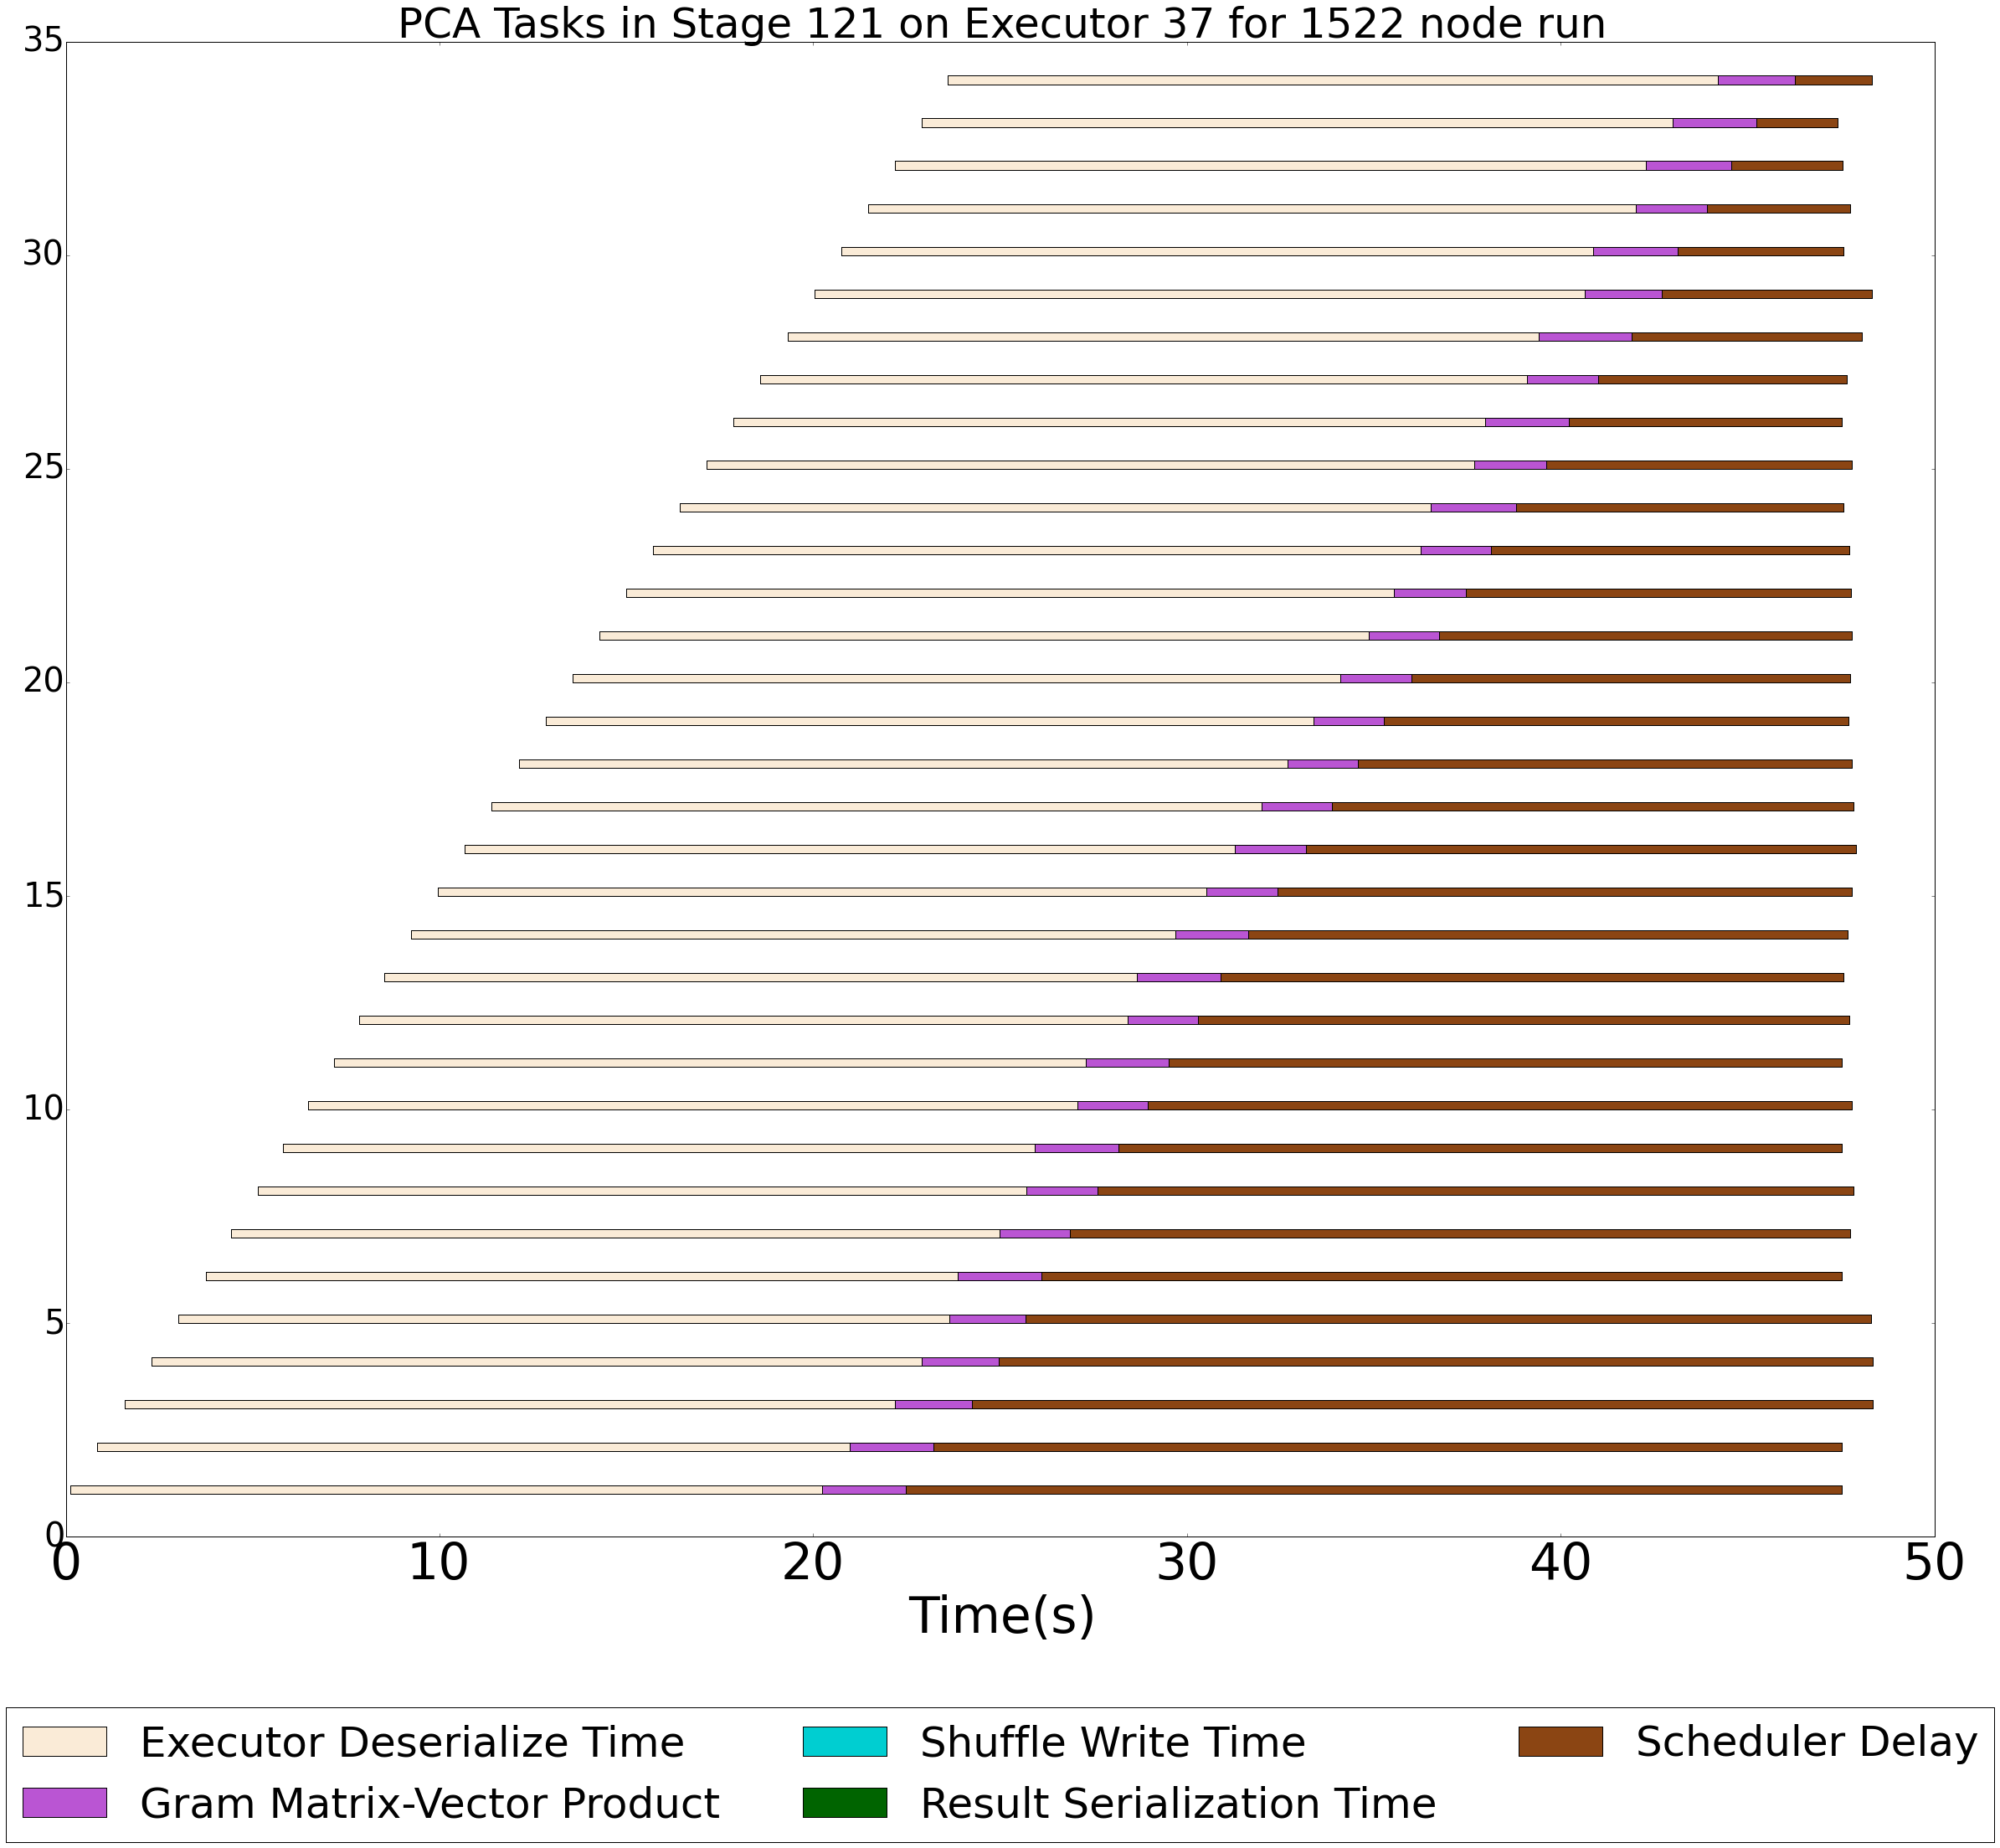
\includegraphics[width=.5\textwidth]{fig/spark_pca_hero_timeline.png}
\caption{A timeline of tasks on a particular node for a multiply Gramian stage during the 1522 node Spark run. }
\label{fig:hero-timeline}
\end{figure}

% \begin{figure}[t]
% 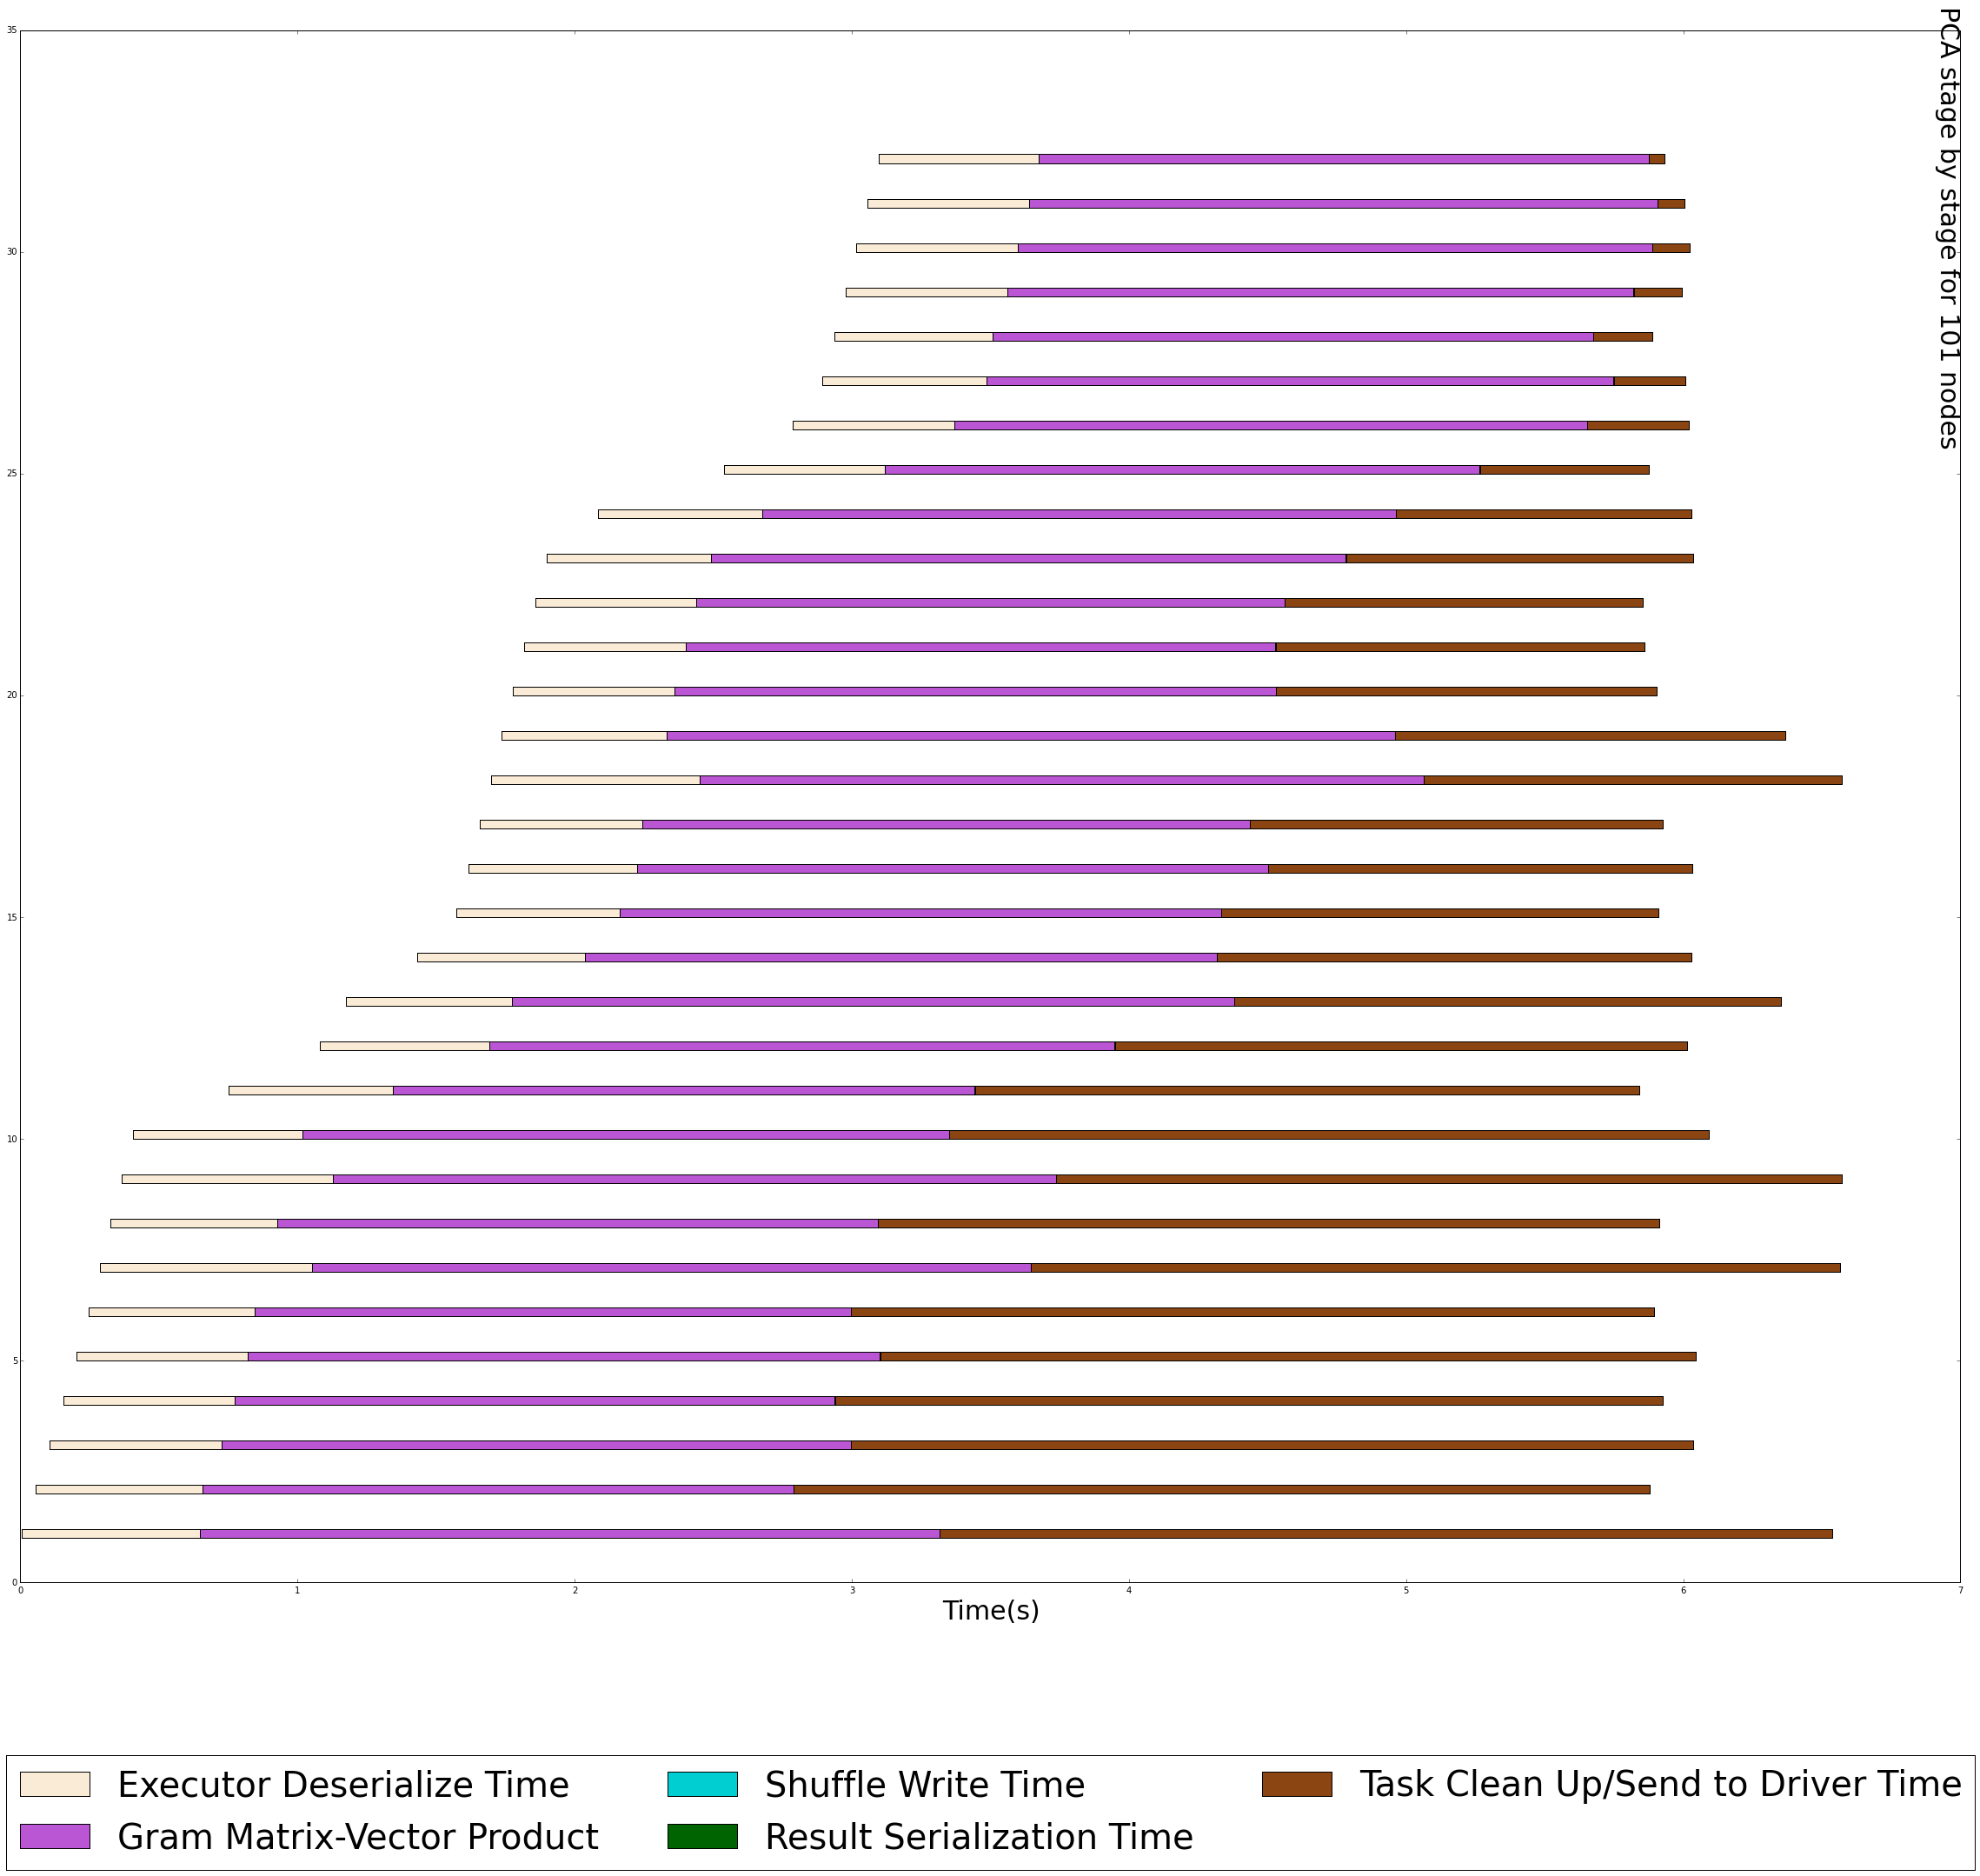
\includegraphics[width=.5\textwidth]{fig/pca_100_timeline.png}
% \caption{???}
% \label{fig:tofix-1}
% \end{figure}

% \begin{figure}[t]
% 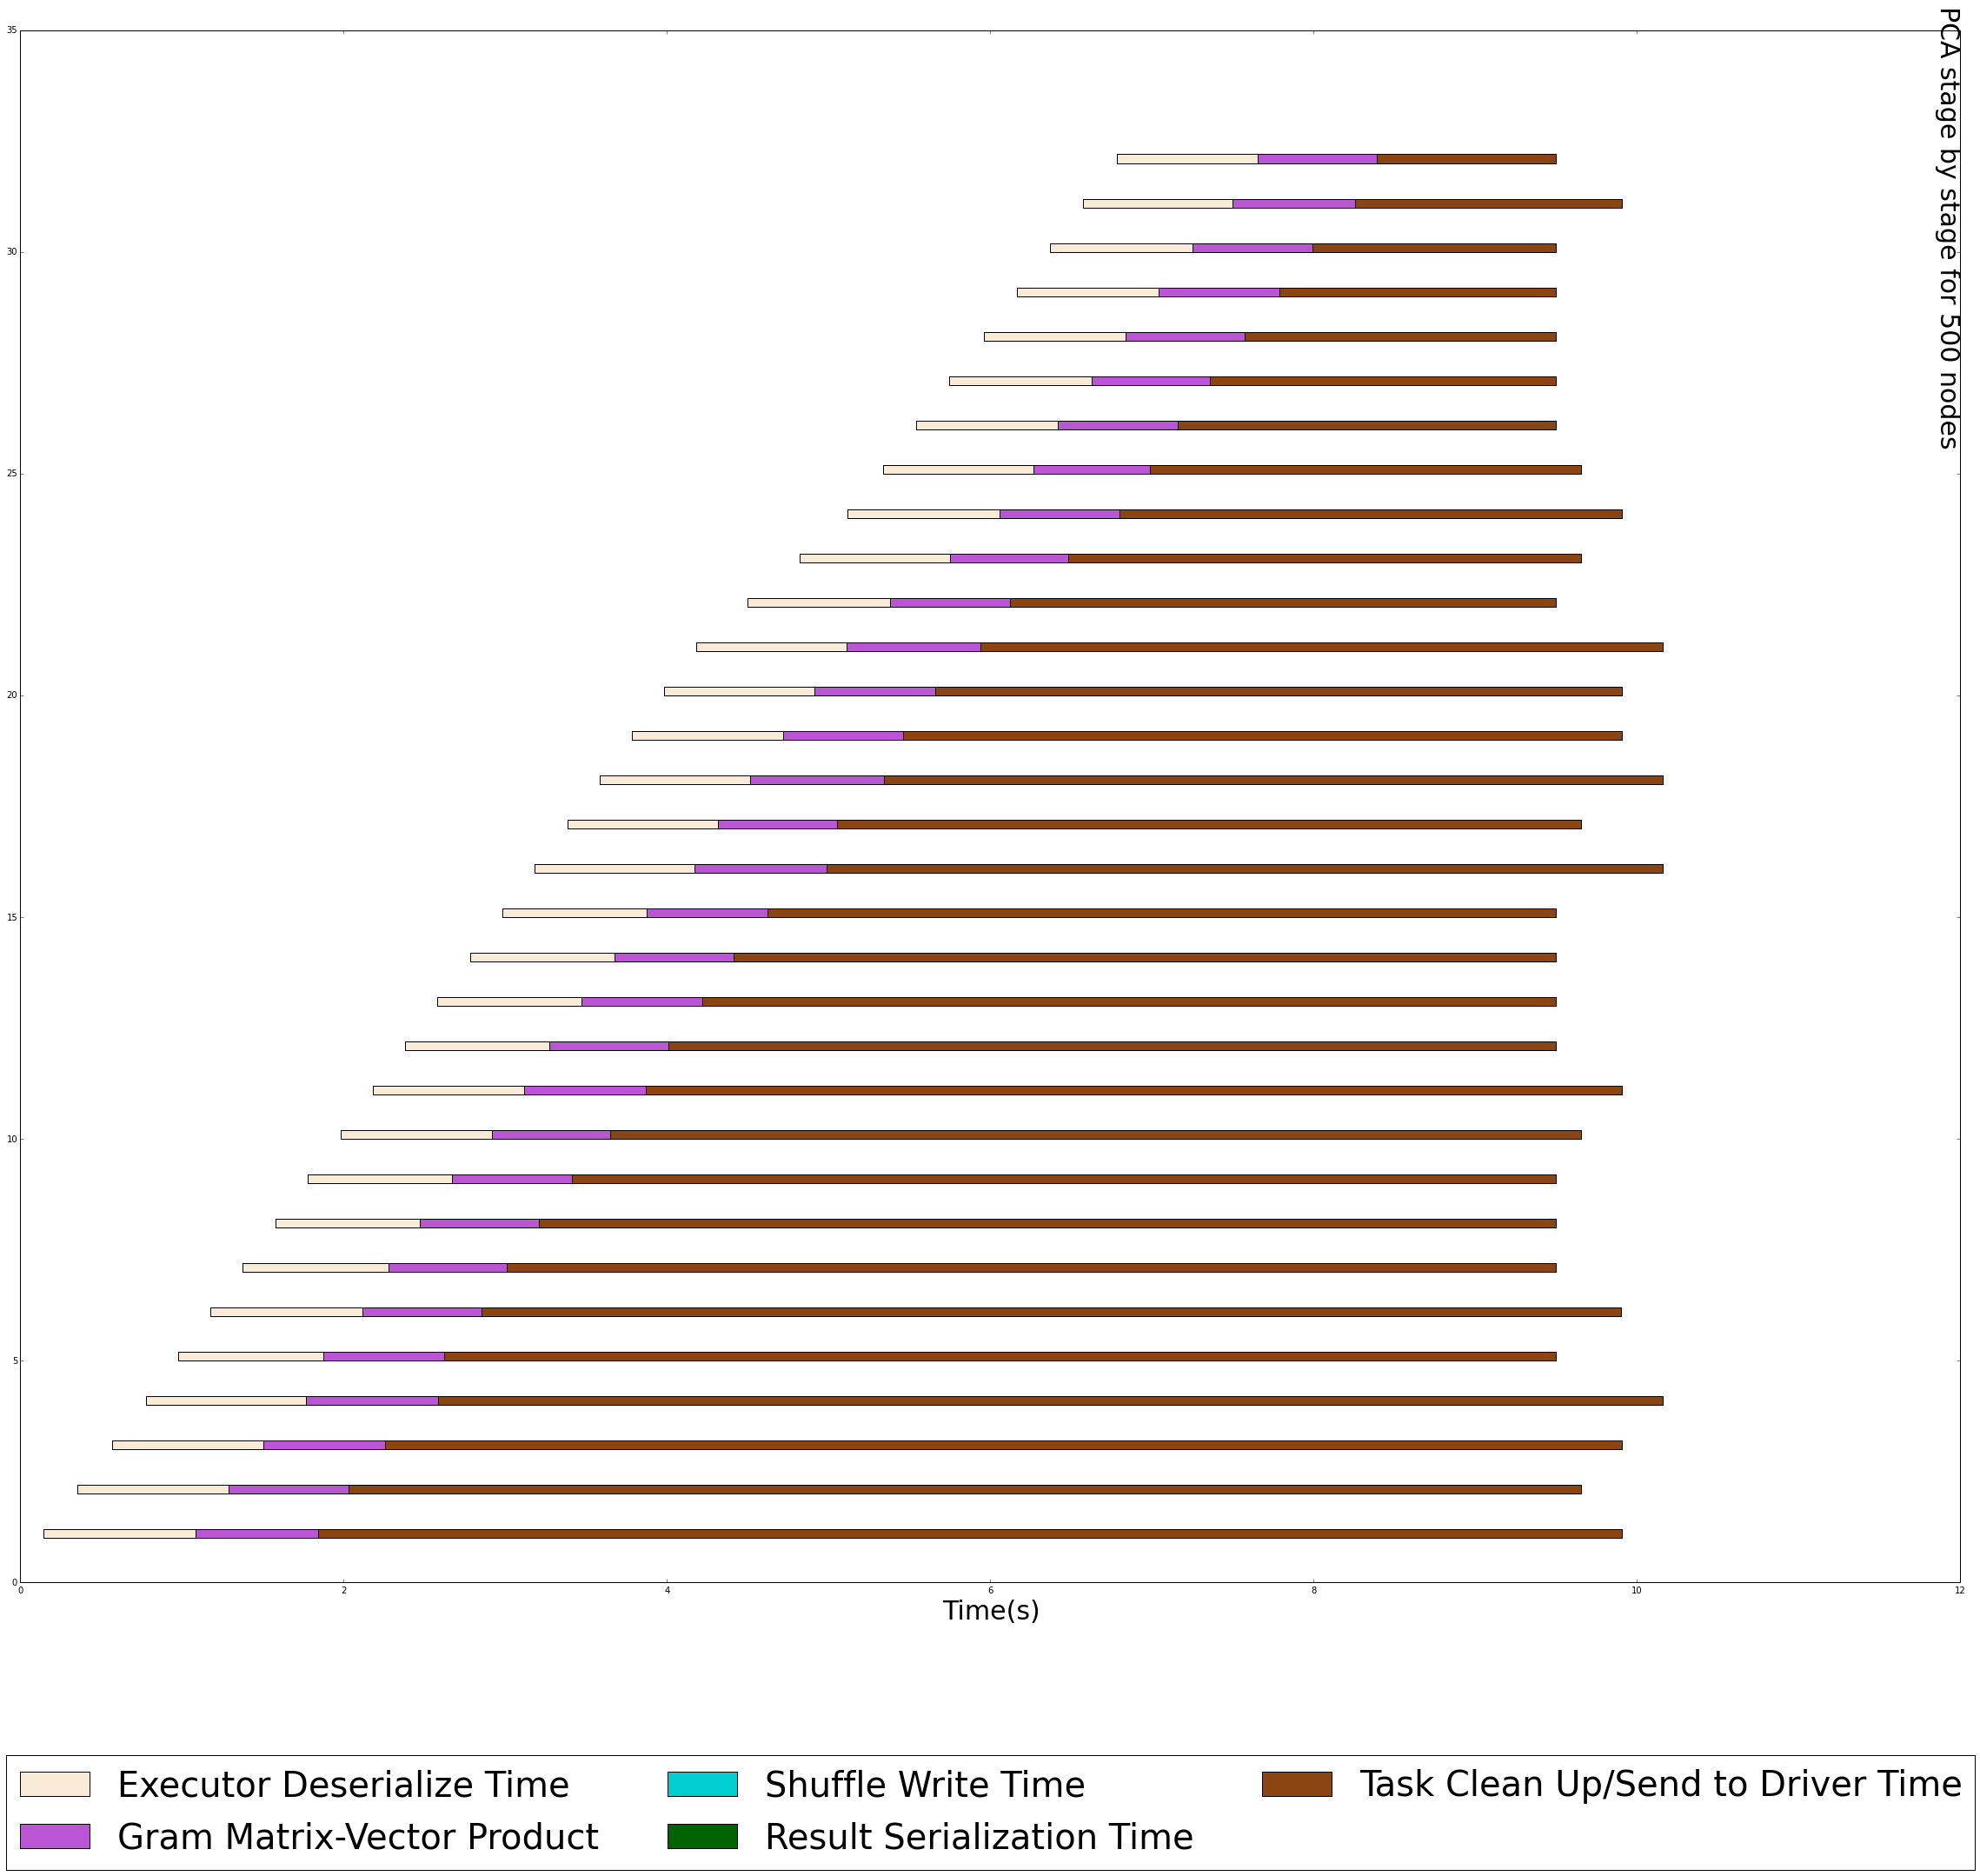
\includegraphics[width=.5\textwidth]{fig/pca_500_timeline.png}
% \caption{???}
% \label{fig:tofix-2}
% \end{figure}

% \begin{figure}[t]
% 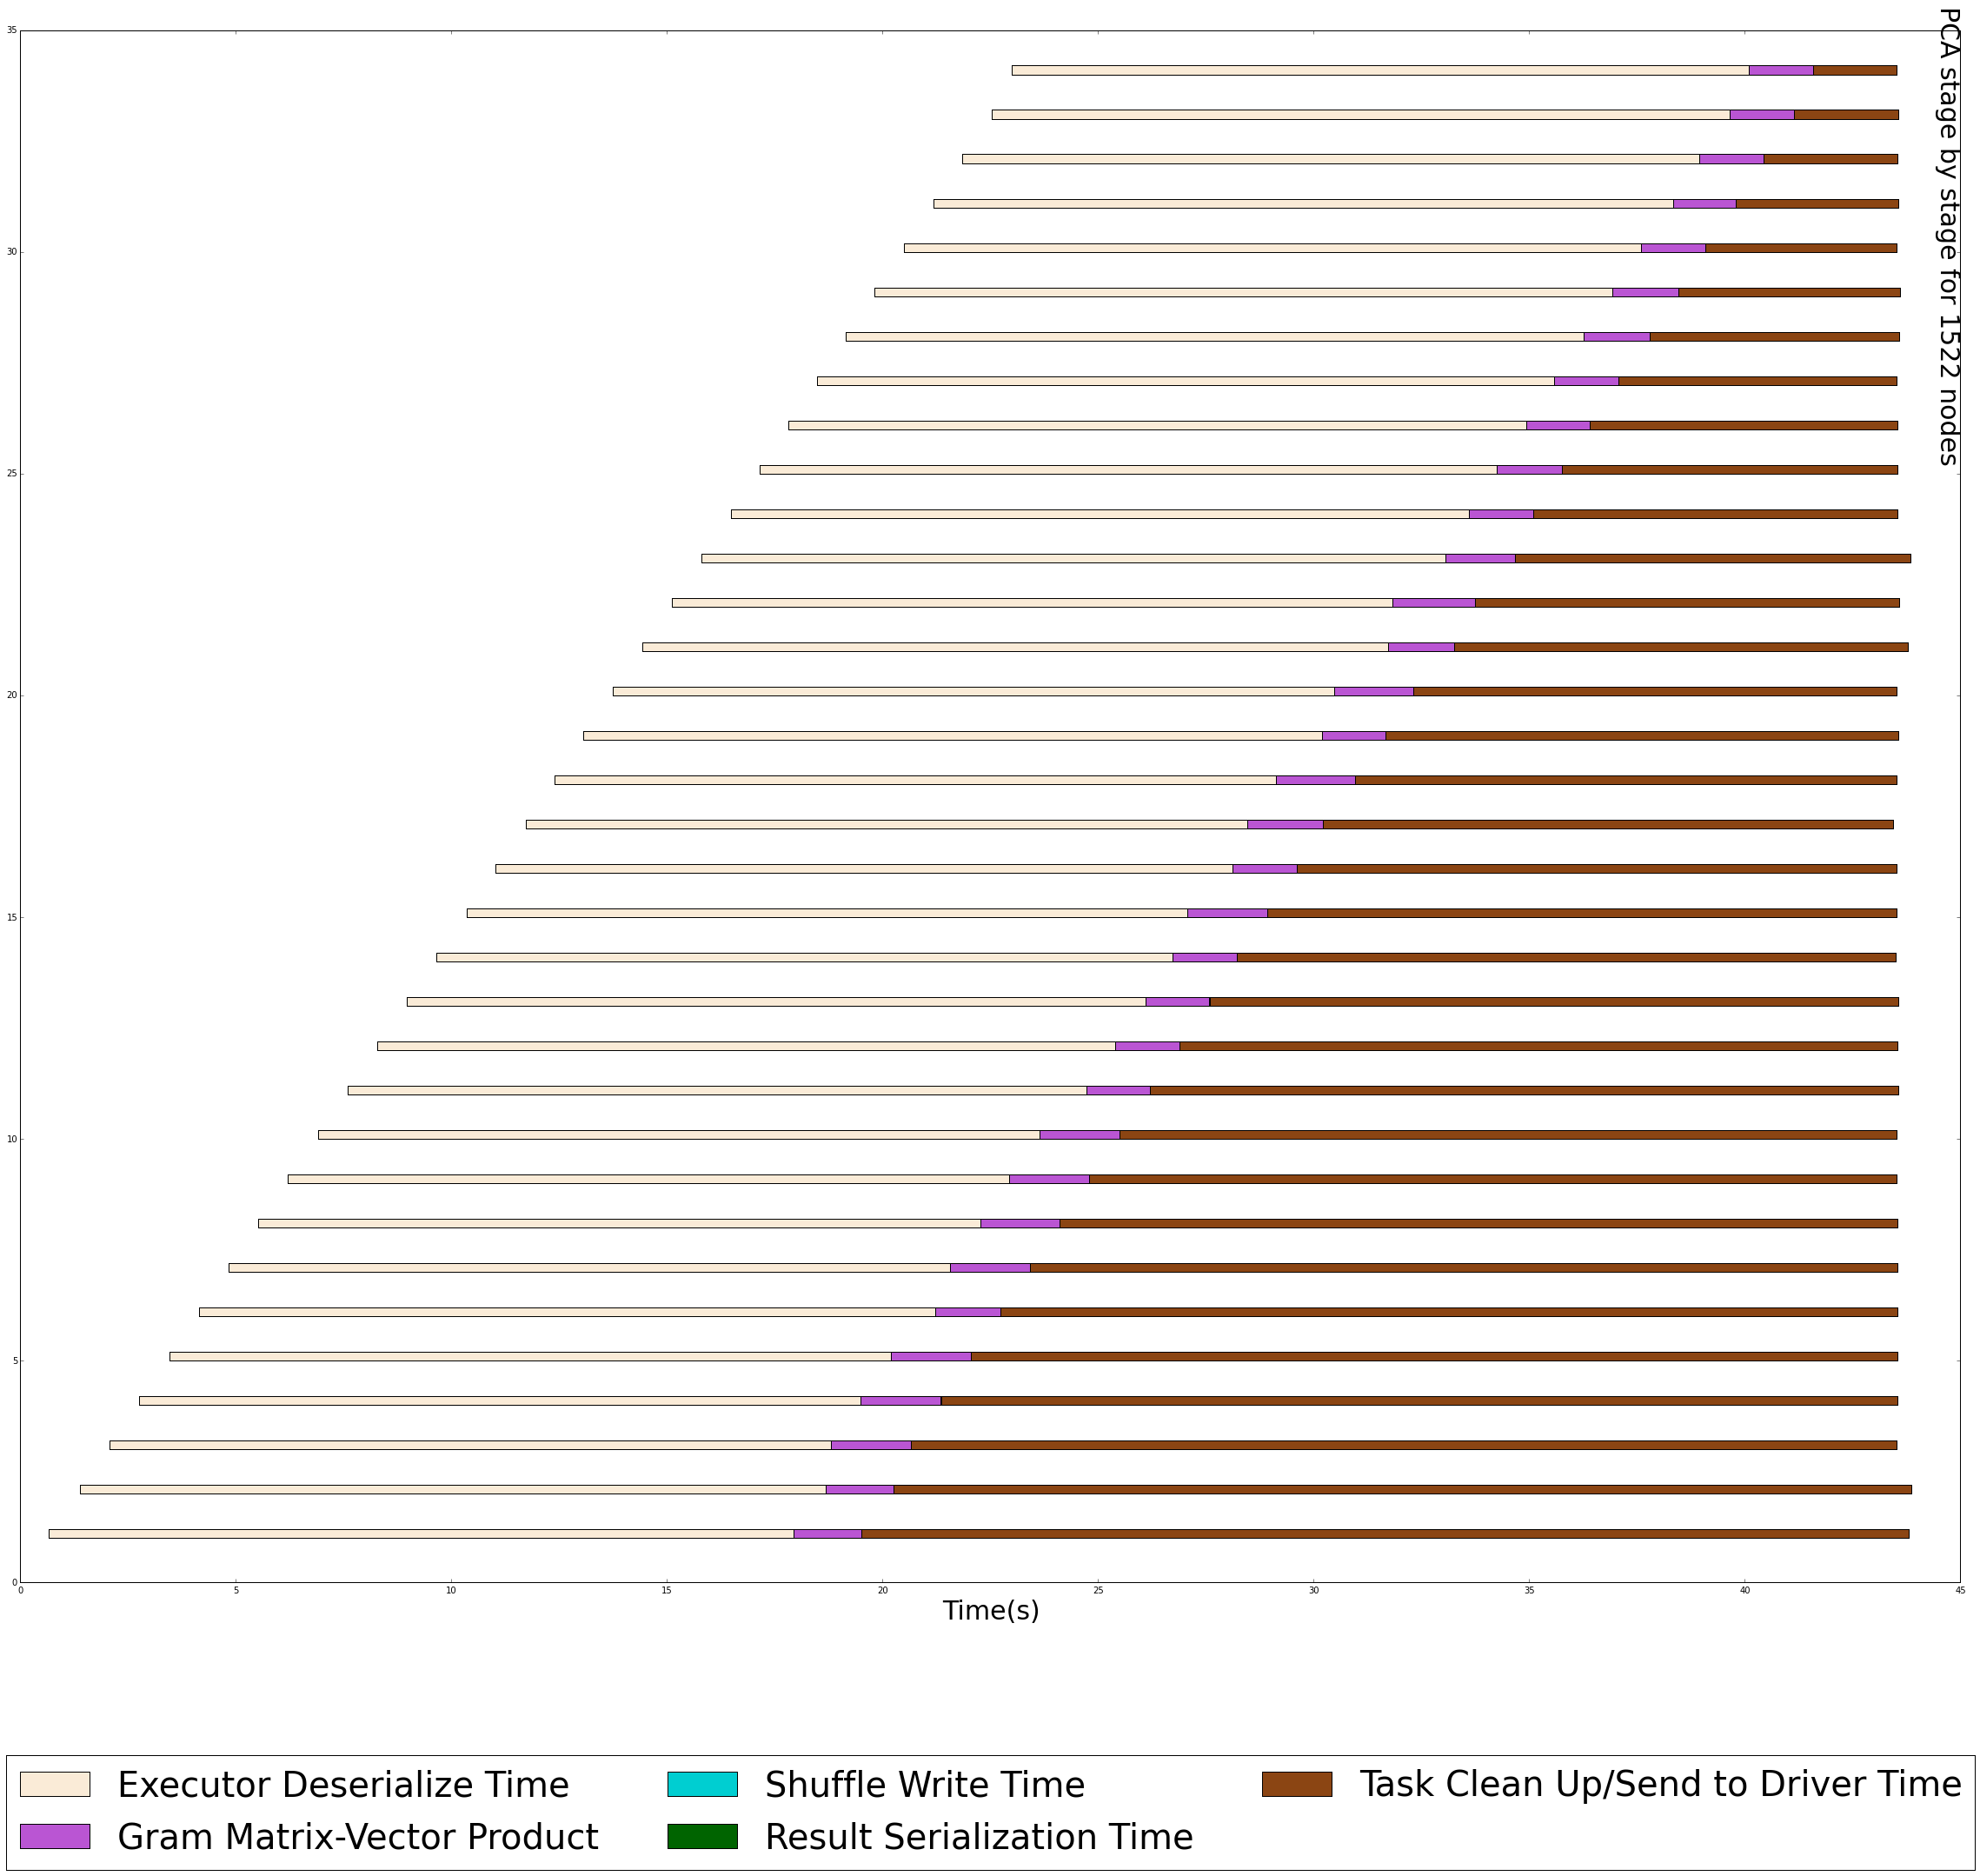
\includegraphics[width=.5\textwidth]{fig/pca_hero_timeline.png}
% \caption{???}
% \label{fig:tofix-3}
% \end{figure}

% \begin{figure}[t]
% 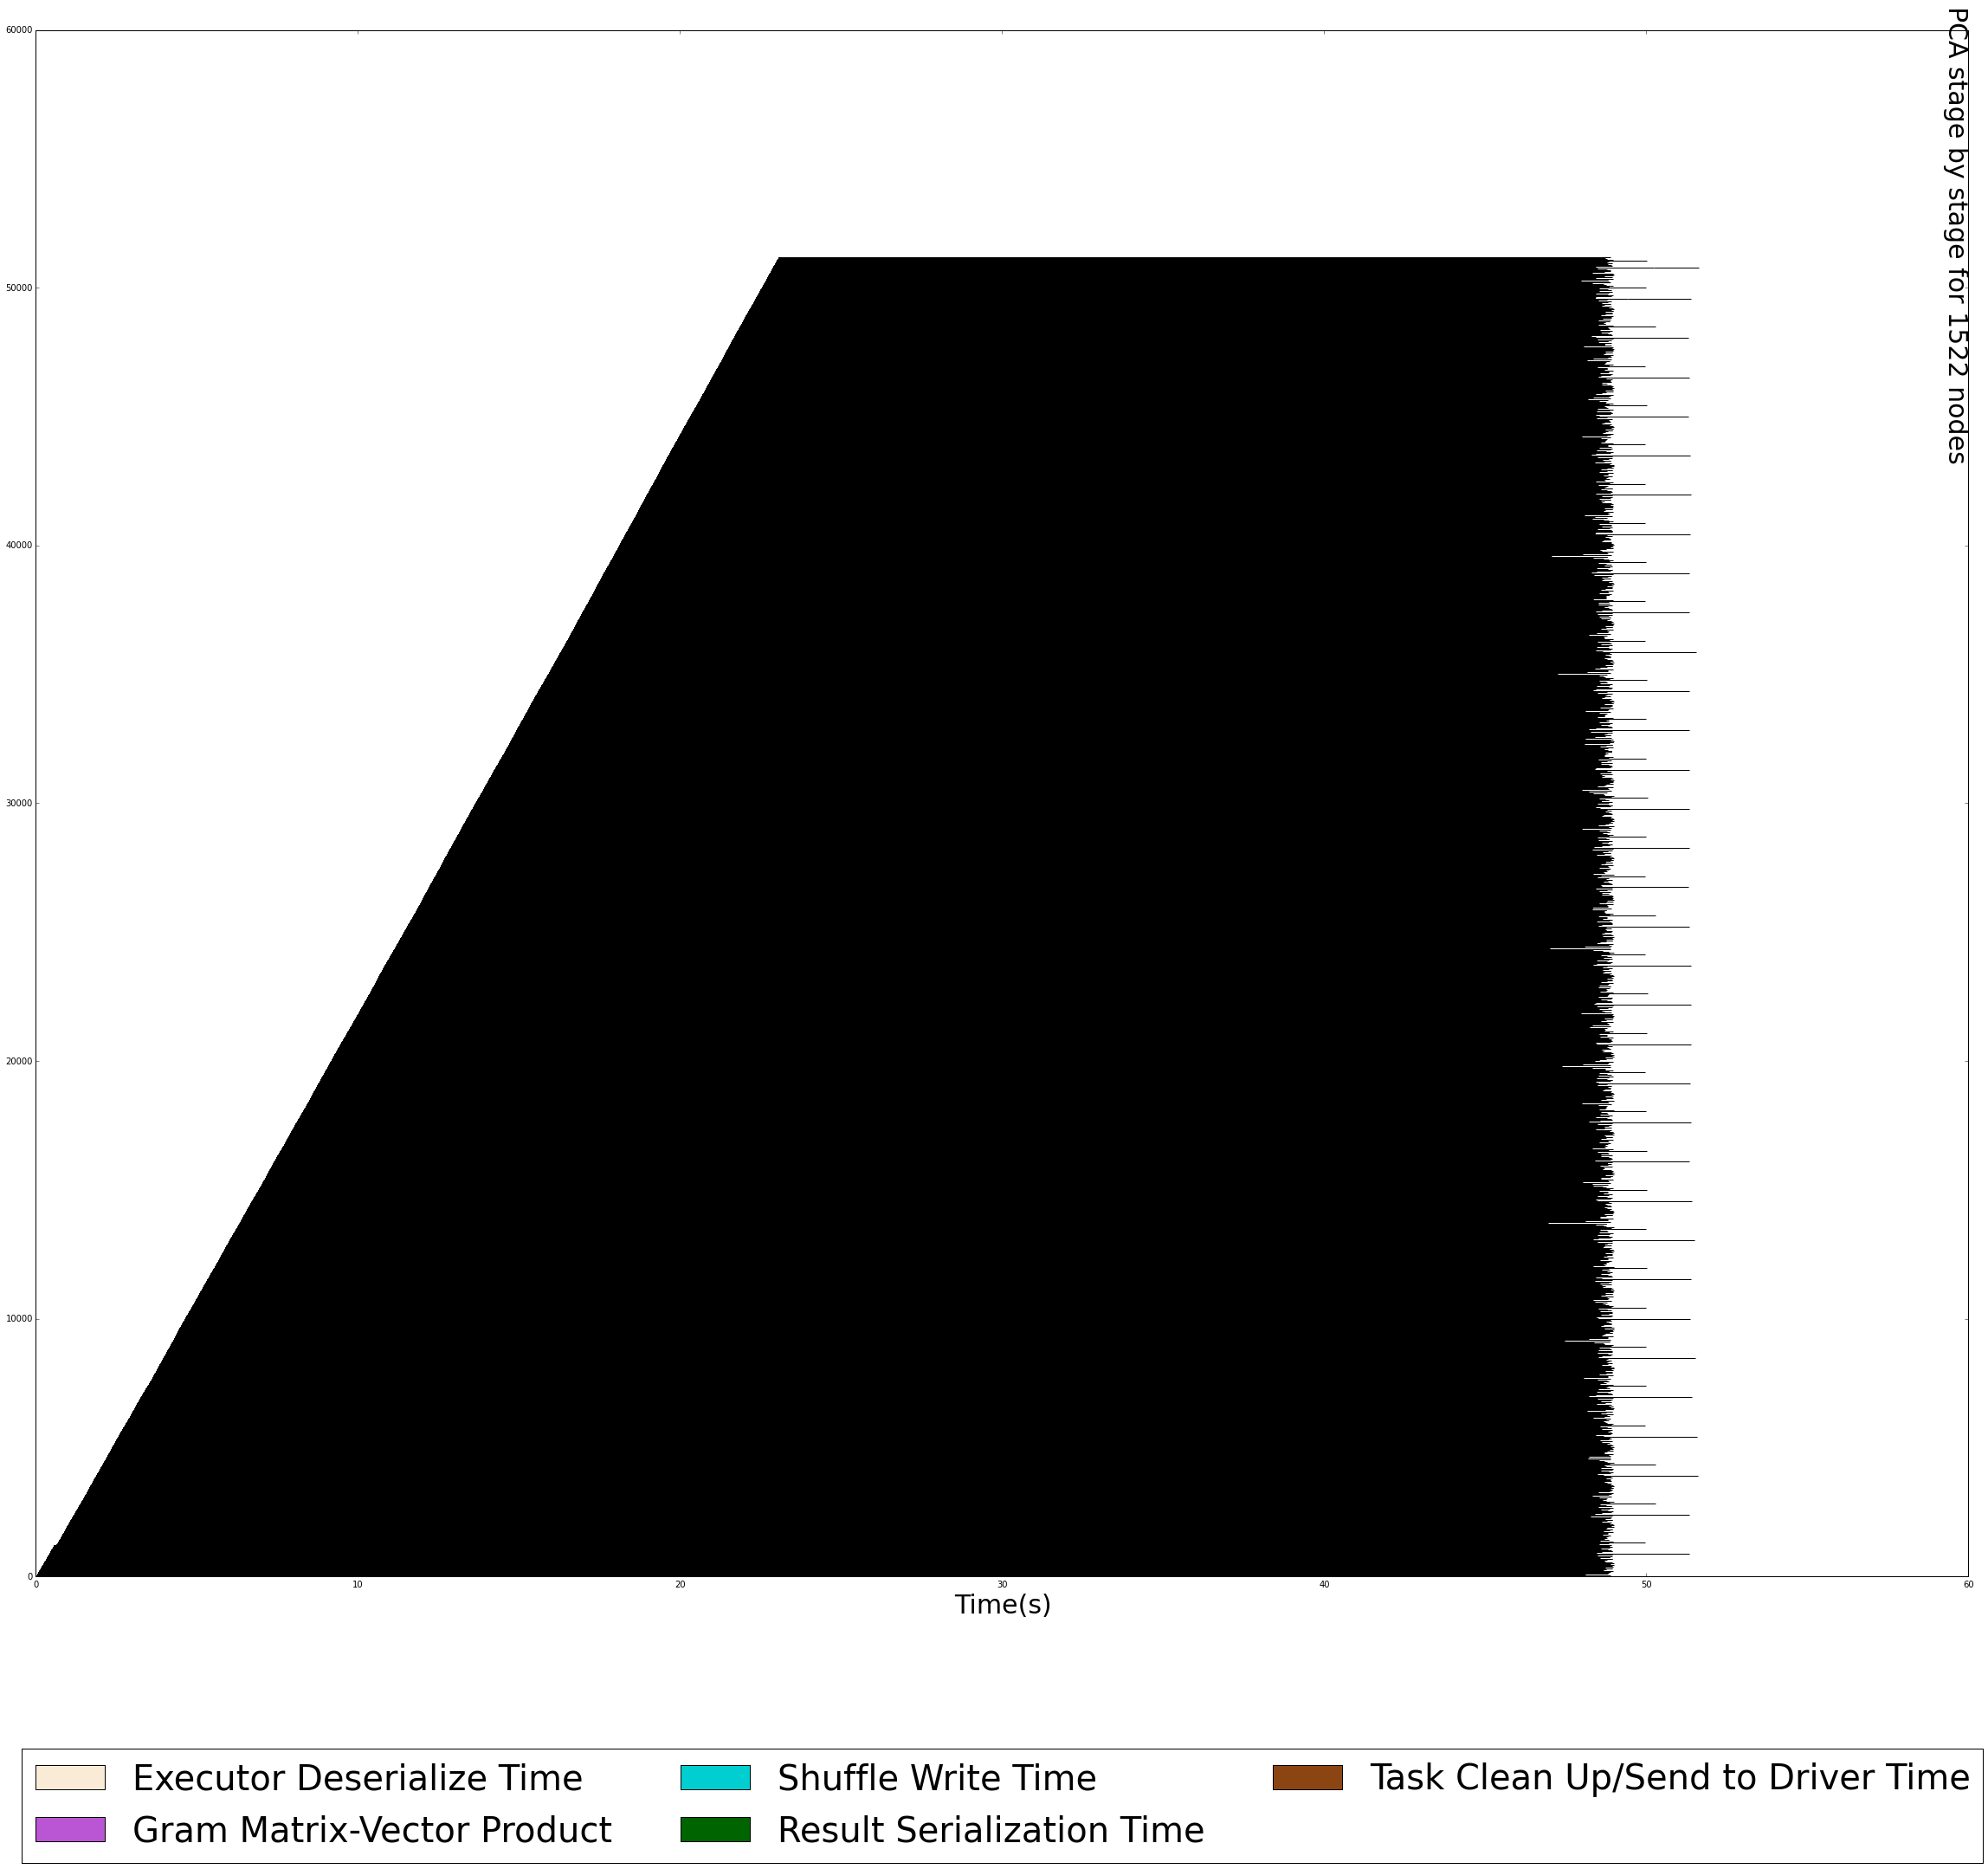
\includegraphics[width=.5\textwidth]{fig/stage7_hero_run.png}
% \caption{???}
% \label{fig:tofix-4}
% \end{figure}

\begin{figure}[t]
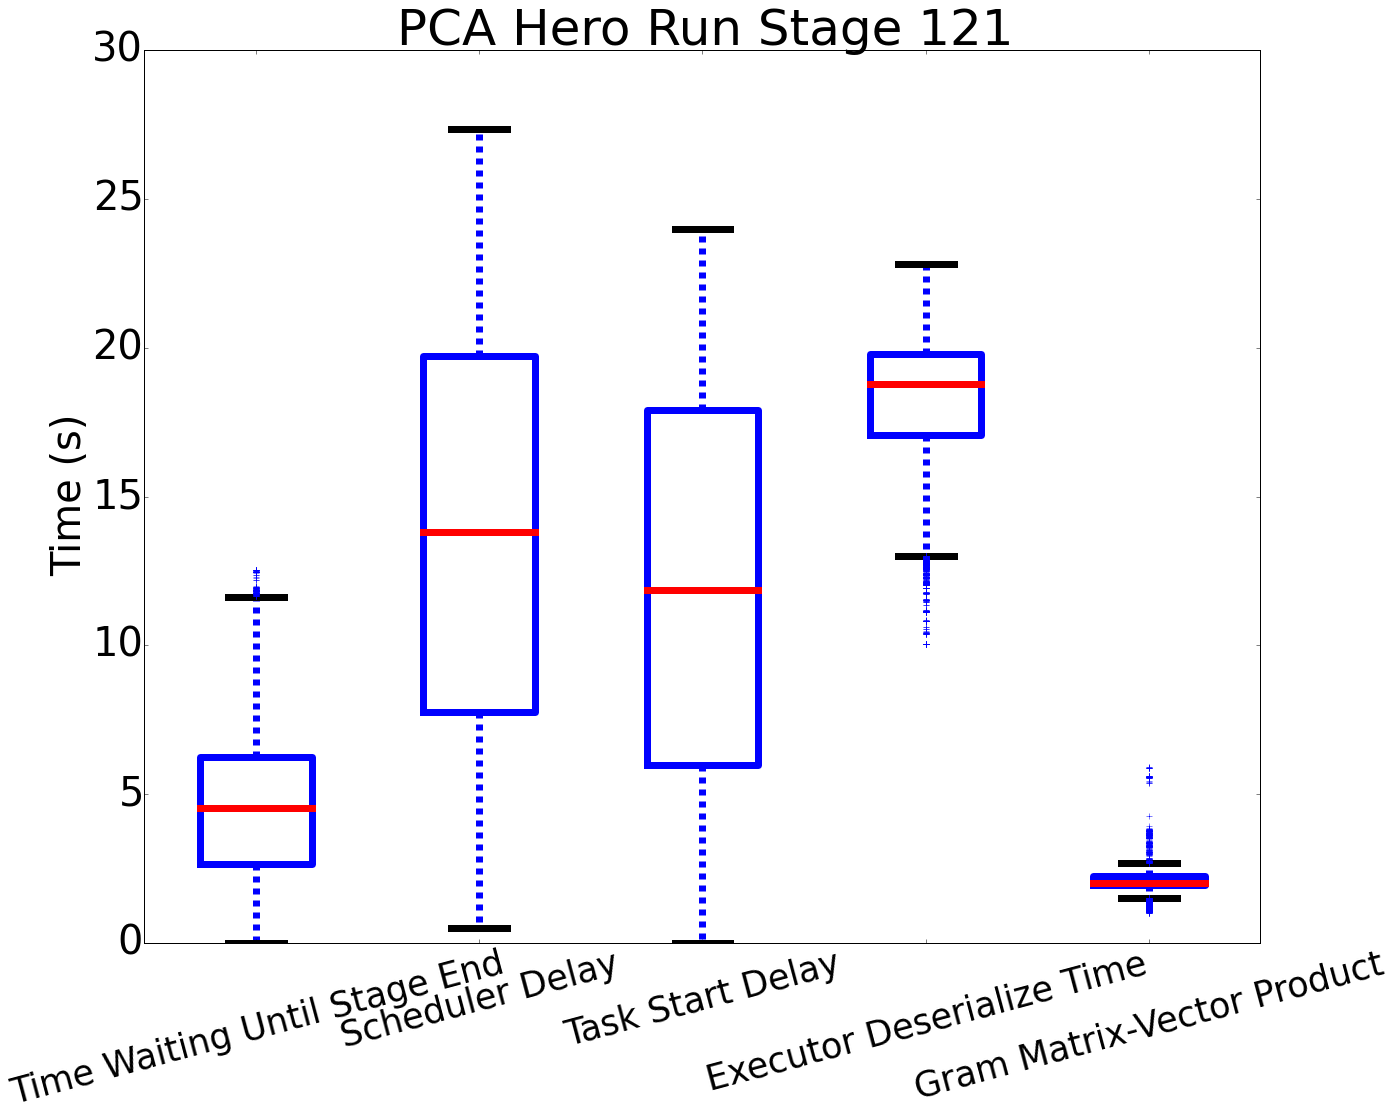
\includegraphics[width=.5\textwidth]{fig/pca_box_and_whiskers.png}
\caption{Distribution of various components of all tasks in a multiply Gramian stage in the Spark PCA hero run. }
\label{fig:whisker}
\end{figure}


